

\section{Introduction}
RML (RDF Mapping Language) and SPARQL (SPARQL Protocol and RDF Query Language) are two important tools in the construction of knowledge graphs and the Semantic Web.
RML is an RDF-based language used for mapping data from different sources to RDF. It allows developers to transform and integrate data from various formats such as CSV, JSON, and XML into RDF triples.
SPARQL is an expressive query language used to retrieve data from RDF triple stores. Its federated query feature allows developers to write complex queries that can retrieve data from multiple sources.
%Together, RML and SPARQL play a crucial role in the construction of knowledge graphs, which are used to represent and interlink data from multiple sources, creating a more comprehensive view of a particular domain.
%As the amount of data on the web continues to grow, the use of RML and SPARQL is becoming increasingly important for
%enabling 
%the creation of large knowledge graphs.
%powerful applications.
So far, both approaches are treated as different: On the one hand there are tools specifically for
processing RML whereas on the other hand there are tools that extend SPARQL in order to incorporate additional data sources.
The motivation for this work is to devise a unified approach to the problem of large-scale knowledge graph construction.
%One of our visions is to enable research into the extent to which findings from SPARQL (query) execution optimizations can be leveraged for RML and vice versa.

The contributions of this work are: (1) We present an approach to translate RML to SPARQL with corresponding optimizations.
(2) We introduce the \emph{Not Only RDF SPARQL Extensions} (NORSE) for processing CSV, JSON and XML.
%JenaX features several extensions that can be plu into Apache Jena's ARQ query engine.
These extensions comprise additional functions and special SERVICE implementations with IRIs in the ``\texttt{norse:}'' namespace \texttt{https://w3id.org/aksw/norse\#}.
 The implementations are part of our JenaX resource\footnote{\url{https://github.com/Scaseco/jenax}} which is available on Maven Central. It features several unofficial extensions for the Apache Jena framework.
(3) We furthermore present an Apache Spark-based SPARQL engine that executes NORSE-enhanced SPARQL by leveraging its massive parallel processing model. We show that performance- and scalability-wise this approach surpasses the state of the art in several scenarios.
It is worth noting that achieving these results is not the sole merit of Apache Spark, but also that of the optimizations we used.

The remainder of this paper is structured as follows:
We present related work
%about mapping languages and tools in the knowledge graph domain
in~\Cref{sec:related-work}.
The translation of RML models to extended SPARQL CONSTRUCT queries is described in~\Cref{sec:rml-to-sparql}.
Optimizations of query workloads with respect to the uniqueness and ordering of the produced RDF triples and/or quads are shown in~\Cref{sec:optimize}.
In \Cref{sec:implementation} we present our implementations for (1) converting RML to SPARQL (2) the NORSE SPARQL extensions
% for Apache Jena's ARQ query engine
and (3) the implementation of a SPARQL engine on Apache Spark using the SANSA Big Data RDF framework.
Subsequently, in~\Cref{sec:eval} we present an evaluation of our approach based on the GTFS Madrid Bench and one dataset of the SDM Genomic Datasets.
%We also discuss which parts of our approach have not yet worked ideally.
We conclude our paper in~\Cref{sec:conclusions}.

The implementation of our approach is part of our RDF Processing Toolkit (RPT)\footnote{\url{https://github.com/SmartDataAnalytics/RdfProcessingToolkit}} which is based on JenaX.

%and point out future work.
%\todo{Provide a link to the tool here}

\section{Related Work}
\label{sec:related-work}
In this section we provide an overview of contemporary SPARQL and RML based knowledge graph construction approaches 
%mapping languages, RML processors, %benchmarks 
as well as a brief summary of Apache Spark.
As there exist many mapping languages\cite{Meester2019, ChavesFraga2021, IglesiasMolina2022a, Assche2023}, a discussion of general concepts and translations between them can be found in \cite{Corcho2020, IglesiasMolina2022}.

%\citet{Corcho2020} and \citet{IglesiasMolina2022}.
%Mapping of data to RDF graphs is usually either done with custom implementations, direct mappings, or using dedicated mapping languages\citep{Dimou2020}. 

%and the parallelization framework Apache Spark.

%\subsection{Mapping Languages}
\subsection{SPARQL-based Mapping Approaches}
%In this article we are focusing on later and especially R2RML\footnote{\url{https://www.w3.org/TR/r2rml/}}, RML\cite{Dimou2014} and SPARQL.
%\todo{I hope I replaced sparql integrate with NORSE correct. Lars-Peter}.
%There are several articles \citep{Meester2019, ChavesFraga2021, IglesiasMolina2022a, Assche2023} on the different mapping languages.
% The most relevant seem to be R2RML\citep{Das2012}, RML\citep{Dimou2014}, SPARQL Generate\citep{lefranccois2017sparqlgenerate}, YARRRML\citep{heyvaert2018declarativeyarrrml} and ShExML\citep{GarciaGonzalez2021}.
%\subsection{R2RML and RML}
%\todo{cite our ldow 2015 paper}.
%R2RML and RML are categorized by  \citet{IglesiasMolina2022a} as "RDF-based".
%Beside the "RDF-based"\cite{IglesiasMolina2022a} R2RML and RML we want to outline SPARQL. 
%\subsection{SPARQL}
%is a recursive acronym for \emph{SPARQL Protocol and RDF Query Language} and
\emph{SPARQL} is a W3C standard for processing (loading, retrieving, transforming and updating) RDF data\footnote{\url{https://www.w3.org/TR/sparql11-query/}}.
%Consequently, \emph{SPARQL engines} are systems that can evaluate \emph{SPARQL statements}.
SPARQL engines can be leveraged to build advanced features on top.
%feature extension points.
Two prominent representatives of the category of SPARQL-based mapping approaches are SPARQL-Generate\cite{lefranccois2017sparqlgenerate} and SPARQL Anything\cite{10.1145/3555312sparqlanything}.
SPARQL Anything extends SERVICE evaluation such that references to remote non-RDF data can be made. The data is converted to an opinionated RDF graph (as per documentation) which then serves as the base for evaluating the remainder of the SERVICE clause.
%It is noteworthy that as an effort to
SPARQL-Generate features a SPARQL-based template language which can produce output beyond what is possible with conventional SPARQL.

Our JenaX project compares to these approaches as follows: JenaX provides (among other things) SPARQL plugins for the Apache Jena ecosystem that allow for processing heterogeneous data within the SPARQL syntax already supported by the framework.
As part of this effort we contributed a plugin system to facilitate interoperability of custom SERVICE execution implementations\footnote{\url{https://github.com/apache/jena/pull/1388}}. 
The SPARQL extensions for processing RML sources, as described in this paper, are built on this system.
While some of JenaX's SPARQL extension functions for XML, JSON and CSV processing conceptually overlap with those provided by SPARQL-Generate, there are yet differences in the implementations. For example, JenaX provides dedicated RDF datatype implementations that internally retain JSON and XML data in an object model, whereas SPARQL-Generate (as of version 2.0.12) falls back to string representations.
In order to avoid clashes we use IRIs in the \emph{norse} namespace for our implementations.

%functions in SPARQL-Generate (2.0.12) always (re-)parse XML and JSON data from string whereas
%SPARQL-Generate (2.0.12) functions
%For example, JenaX supports dedicated RDF datatype implementations that internally retain JSON and XML data in an object model.  SPARQL-Generate (2.0.12) functions
%For example, JenaX supports dedicated RDF datatype implementations for JSON and XML that internally store the data in an object model which can be leveraged and the performance characteristics.
%For example, JenaX provides RDF datatype implementations that internally store JSON and XML in an object model in order to allow for fast operations whereas SPARQL-generate functions so far currently parse and produce strings.
%For example, JenaX features specialized RDF datatype implementations that internally represent JSON and XML in an object model rather than strings. 

%\todo{finish}
%The \emph{Not Only RDF SPARQL Extensions} (NORSE) SPARQL extensions introduced in \Cref{sec:NORSE} add support for CSV and JSON input.
%There are several ways to express extensions:\addtocounter{footnote}{-3} %3=n
%\stepcounter{footnote}
%Magic triples, Comments (\#pragma) RDF Reasoning in stardog.

\subsection{RML Processors and Benchmarks}
\emph{R2RML} is a W3C standard and vocabulary for mapping relational data to RDF\footnote{\url{https://www.w3.org/TR/r2rml/}}.
On the one hand these mappings can be used in ETL processes to dump databases as RDF. On the other hand, the same mappings can be used in SPARQL-to-SQL rewriting, a.k.a. OBDA (ontology-based data access). While R2RML is considered quite verbose, several alternatives have been developed, such as the Stardog Mapping Syntax (SMS, currently in version 2), the Ontop Mapping Language\cite{calvanese2017ontop}, and the Sparqlification Mapping Language\cite{stadler2015simplified}.

\emph{RML}\footnote{\url{https://rml.io/specs/rml/}} is an extension of R2RML which adds additional vocabulary for mapping non-relational data\citep{Dimou2014, Dimou2020}. In essence these additional declarations allow for expressing a mapping of non-relational data (such as XML and JSON) into a relational model where from each row RDF tuples are generated. Like R2RML it suffers from verbosity, for which reason simplified models were derived such as YARRRML\cite{heyvaert2018declarativeyarrrml}.
A mapping translation between ShExML\cite{GarciaGonzalez2021} and RML is presented by \cite{GarciaGonzalez2022}.

There exist several RML processors \cite{ArenasGuerrero2021, Iglesias2023}\footnote{\url{https://github.com/kg-construct/awesome-kgc-tools}} for the well known extension RML of the W3C standard R2RML. 
%\citet{ArenasGuerrero2021} gives an overview on the state of the art and compares them using the Madrid GTFS benchmark.
%\citet{Iglesias2023} introduces some optimization and compares the RML processors RMLMapper, RocketRML, Morph-KGC and SDM-RDFizer using the Madrid GTFS benchmark and the SDM-Genomic-Datasets.
In this paper we are comparing benchmarks with the following: %Morph-KGC and SDM-RDFizer.
\emph{SDM-RDFizer}\footnote{\url{https://github.com/SDM-TIB/SDM-RDFizer}} is an RML processor implemented in python with optimized data structures and operators. It is developed with scalability and complex data in mind\cite{Iglesias2020}.
\emph{CARML}\footnote{\url{https://github.com/carml/carml}} and RMLMapper\footnote{\url{https://github.com/RMLio/rmlmapper-java}} are Java implementations which operate single threaded at the time of writing.
% TODO \emph{RMLStreamer} is a Flink-based implementation however upon writing the standalone container would not work so we deployed it on a cluster but on GTFSbench it would suffer from the missing self-join elimination. We decided to only benchmark the tools that could be used standalone.
\emph{Morph-KGC}\footnote{\url{https://github.com/morph-kgc/morph-kgc}} is an RML processor implemented in python and supports partitioning RML assertions\cite{arenas2022morphkgc} for parallel execution.

%and \emph{RMLStreamer}\cite{Haesendonck2019} are Java-based RML mappers.
%making use of input streaming.

%RML-conformance-test
%RML extension for excel
%RMLMapper / RMLStreamer: Similar tools, essentially the latter adds support for streaming input sources.
%Ontop\citep{calvanese2017ontop}


%\subsection{RML processor benchmarks}
For measuring the performance of the RML processors we use the following benchmarks:
The \emph{Madrid GTFS benchmark}\footnote{\url{https://github.com/oeg-upm/gtfs-bench}} was introduced by \cite{chaves2020gtfs}.
It is based on data from subway network of Madrid and the benchmark data can be scaled up.
A survey on RML tools\cite{ArenasGuerrero2021} conducted in 2021 evaluated 3 virtualizers and 6 materializers on the GTFS Madrid Benchmark.
% Madrid GTFS benchmark\footnote{\url{https://github.com/oeg-upm/gtfs-bench}}\cite{chaves2020gtfs} and the SDM-Genomic-Datasets benchmark\footnote{\url{https://figshare.com/articles/dataset/SDM-Genomic-Datasets/14838342/1}}.
The \emph{SDM-Genomic-Datasets benchmark}\footnote{\url{https://figshare.com/articles/dataset/SDM-Genomic-Datasets/14838342/1}} was introduced by \cite{Iglesias2020}.
This benchmark is motivated from the biomedical domain and based on the Catalogue Of Somatic Mutations In Cancer\footnote{\url{https://cancer.sanger.ac.uk/cosmic}}.
    
%\begin{itemize} \label{sec:benchmarks}
    %\label{sec:bench-madrid}

    % The evaluation suggests that at this time no system was capable of running the GTFS1000 benchmark within a 24 hours time limit.
    % This is no longer the case in 2022 work!

%    \label{sec:bench-sdm}

%\end{itemize}

%There are individual evaluations used as well, like the RMLStreamer benchmark suite \footnote{\url{https://github.com/s-minoo/rmlstreamer-benchmark-rust}} used with RMLStreamer\citep{Oo2022RMLStreamerSISO}.

%Berlin Sparql Benchmark: probably not relevant here

\subsection{Apache Spark And SANSA}
Apache Spark\footnote{\url{https://spark.apache.org/}} is a framework for high parallelisation. It can scale workload execution from a single node to big clusters. Apache Spark advanced Hadoop's Map-Reduce paradigm with an abstraction called "resilient distributed datasets" (RDDs).
%\cite{Zaharia2010SparkCC}.
The SANSA framework\cite{lehmann2017distributed} is an effort to enable various forms of RDF processing on Apache Spark.
%\todo{cite lehmann2017distributed as it is referenced nowhere else}

\section{Translating RML to SPARQL}
\label{sec:rml-to-sparql}
In this section we describe our approach to translate RML to SPARQL.
For this purpose we first briefly summarize the notion of a SPARQL CONSTRUCT query.
%In the course of this section we also introduce SPARQL extensions for operating on heterogeneous data which we refer to as \emph{Not Only RDF Sparql Extensions} (NORSE).

\subsection{CONSTRUCT Queries}
A CONSTRUCT query has the form \lstinline|CONSTRUCT { template } WHERE { pattern }|.
Without loss of generality, for this work we assume generalized RDF\footnote{\url{https://www.w3.org/TR/rdf11-concepts/\#section-generalized-rdf}}.
Let there be the pairwise disjoint sets of IRIs $I$, blank nodes $B$ and literals $L$.
The set of \emph{RDF terms} is defined as $T := I \cup B \cup L$. Furthermore, let there be another set of SPARQL variables $V$. We define the set of \emph{SPARQL terms} $S := T \cup V$.
A {concrete} triple is an element of $T \times T \times T$ whereas a triple pattern is an element of $S \times S \times S$.
Likewise, a {concrete} quad is an element of $T \times T \times T \times T$ whereas a quad pattern is an element of $S \times S \times S \times S$.
The current SPARQL standard only allows for a CONSTRUCT template to specify the creation of triples using triple patterns.
However the importance of this issue has been noted\footnote{\url{https://github.com/w3c/sparql-12/issues/31}}
and several engines already support the production of quads as well.
The approach presented in the following can be used in either setting, so instead of talking about a triple and quad (pattern) we generally speak of a \emph{tuple} (pattern).
A construct query's template is thus made up of a set of tuple patterns. Substituting all variables of these tuple patterns with RDF terms thus produces a set of \emph{concrete} tuples.

%\todo{clean up}
%Other mappings available as well:
%general article: \citep{IglesiasMolina2022}
%ShExML to RML: \citep{GarciaGonzalez2022}
%Grafikeidee: yarrrml -> RML, shexml -> RML -> sparql

\subsection{Translating RML Logical Sources}\label{sec:NORSE}
The two main issues that need to be solved are how to translate (1) RML sources and (2) RML references to SPARQL elements.
RML sources conceptually emit a set of records whose attribute access is specified via \texttt{rml:reference}s.
On the SPARQL side, the \texttt{SERVICE} clause can be used to generate a set of bindings based on its contained pattern.
We can thus introduce a special SERVICE IRI \texttt{norse:rml.source} which contains a graph pattern that represents an RML source.
In addition, we add an additional triple pattern with the special predicate \texttt{norse:output} in order to bind the source records as RDF terms to a SPARQL variable.
%\todo{Move, rephrase or remove Paragraph below}
%Unfortunately, at present SPARQL lacks standardization for non-RDF datatypes and functions. Although RDF defines the datatype \texttt{rdf:XMLLiteral}, RDF frameworks
%do not necessarily implement it in a way that allows for e.g. efficient evaluation of XPath expressions\footnote{For example, Apace Jena stores XML literal internally as strings}.
Therefore, we introduce custom XML\footnote{Jena's implementation of the \texttt{rdf:xmlLiteral} datatype only stores XML as a string which is not suited for efficient XPath evaluation.} and JSON datatypes as well as corresponding functions, namely \texttt{norse:json} and \texttt{norse:xml} to capture XML and JSON data efficiently, respectively.


\begin{figure*}[htb]
\centering
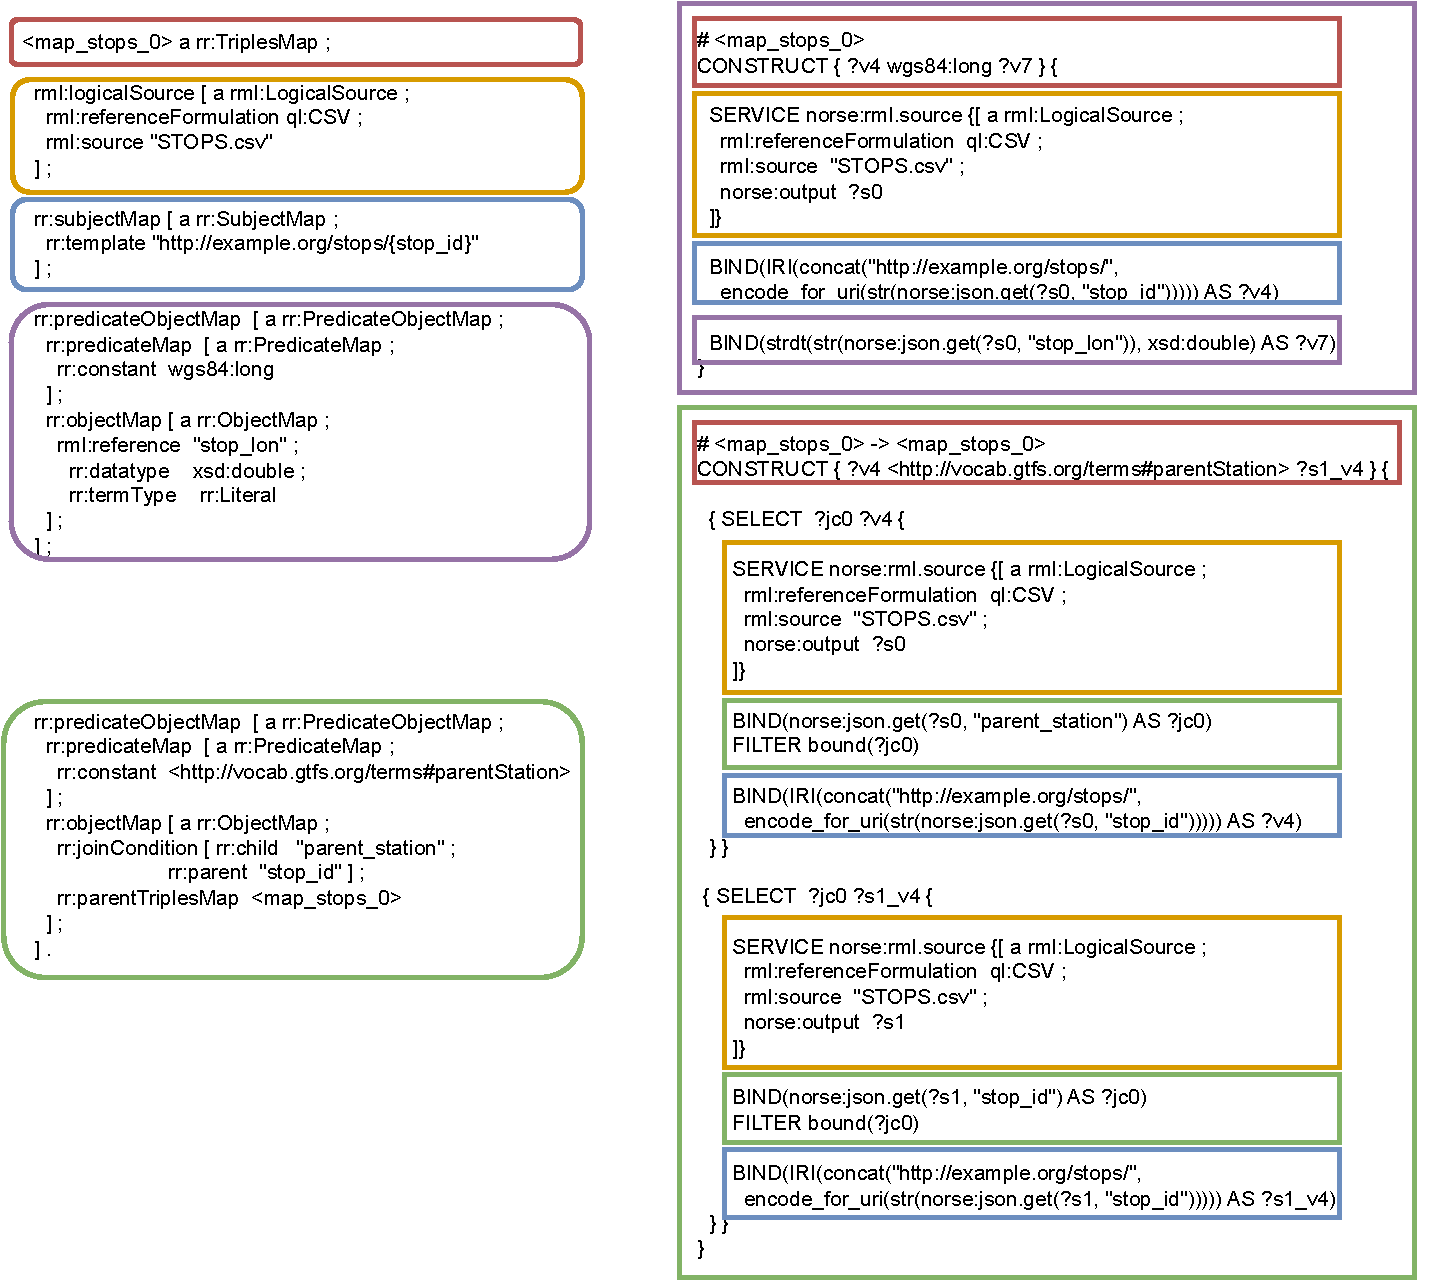
\includegraphics[width=0.9\textwidth]{images/rml-to-sparql.pdf}
%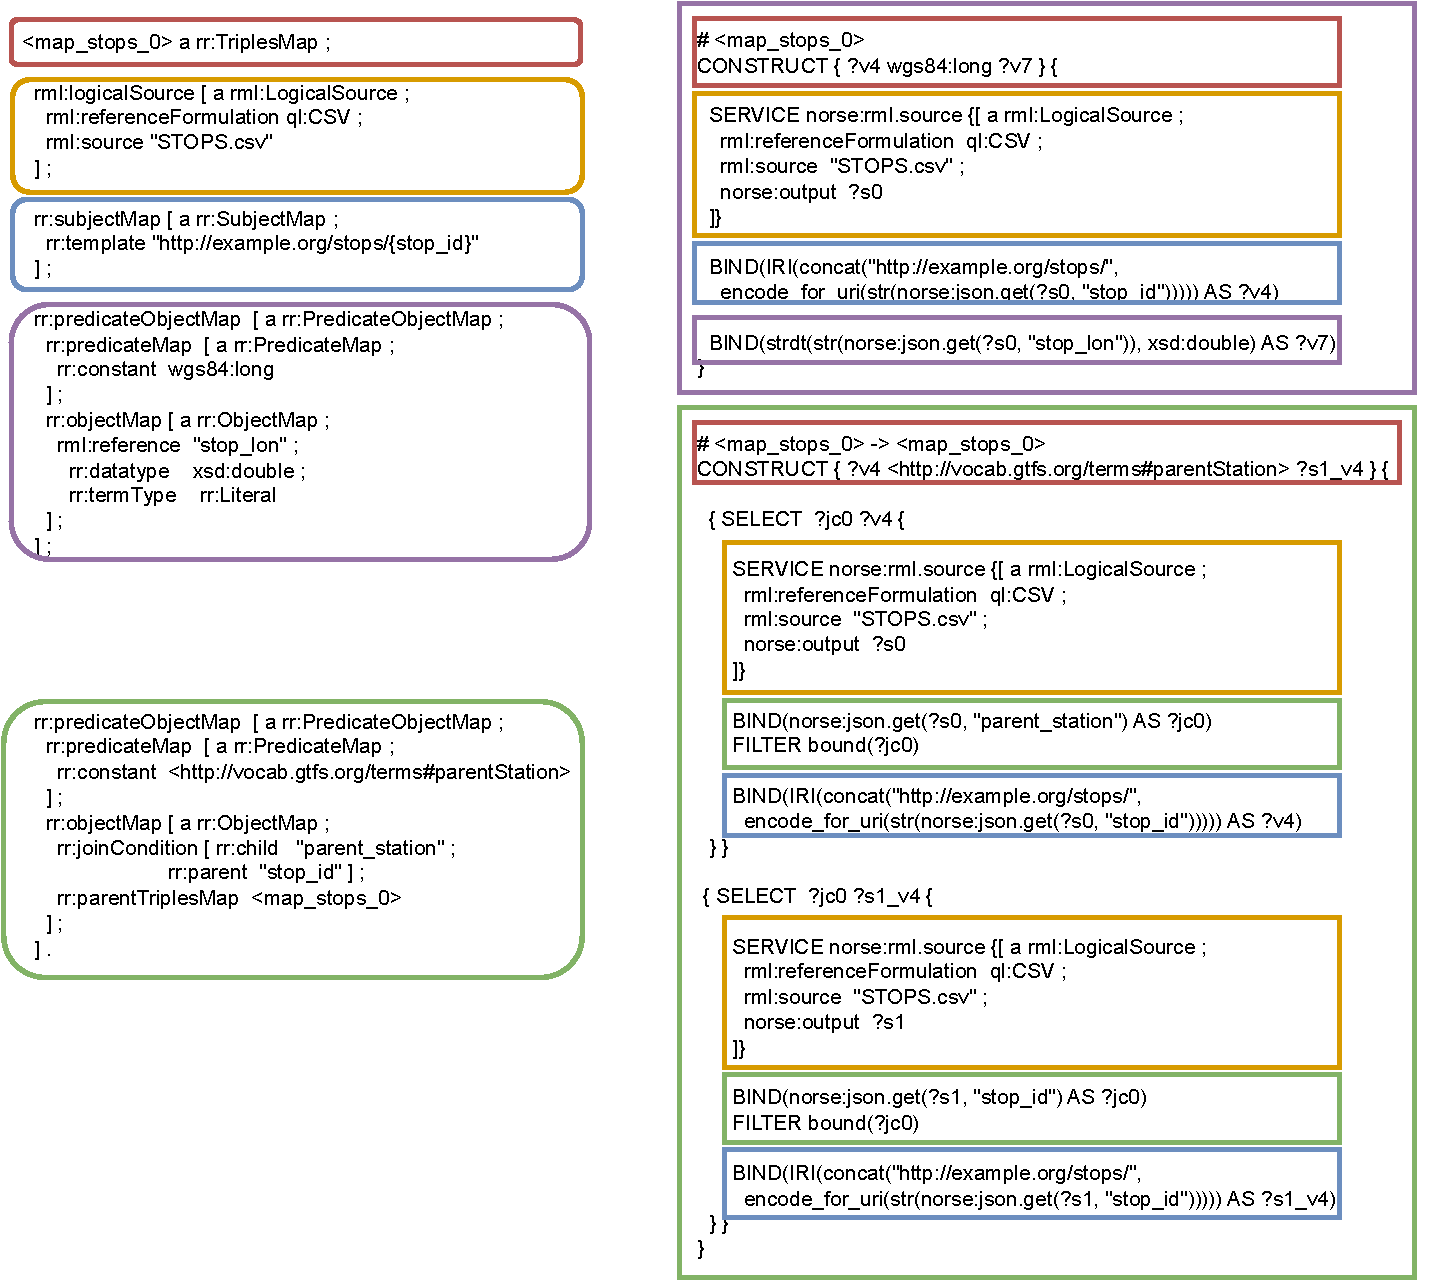
\includepdf[pages=-]{images/rml-to-sparql.pdf}
\label{fig:rml-to-sparql}
\caption{Juxtaposition of an RML document and its representation as SPARQL queries. The RML join condition is transformed into a natural join of SPARQL graph patterns where the same variable (\texttt{?jc0}) is bound on both sides.}
\end{figure*}

\subsection{Translating RML TermMaps}
RML TermMaps specify how to map the referenced data to RDF terms.
SPARQL operates at the level of bindings where variables are bound to RDF terms.
Hence, we can represent RML TermMaps in SPARQL by using \texttt{BIND} to define variables as expressions over a source's data.
SPARQL provides the functions \texttt{IRI}, \texttt{STRDT}, \texttt{STRLANG} and \texttt{BNODE}\footnote{Unfortunately the standard \texttt{BNODE} function is not deterministic so SPARQL-based knowledge graph construction tools typically either alter the semantics or provide an alternative function.} for the construction of RDF terms.
Consequently, every TriplesMap's term map can be represented using a freshly allocated variable that is bound to a corresponding definition using a SPARQL \texttt{BIND} statement. A summary for mapping RML term maps to SPARQL is shown in~\Cref{fig:tm-to-sparql}. The function \texttt{access} is thereby a placeholder that needs to be replaced with a concrete variant based on the type of the logical source (e.g. XML, JSON, CSV) as explained in~\Cref{sec:rml-ref-to-sparql}.

\begin{figure*}
\begin{footnotesize}
\begin{itemize}
%    \setlength\itemsep{-0.5em}
  %\setlength{\itemindent}{.5in}
  \item \lstinline{[ rr:reference "ref" ]} $\rightarrow$ \lstinline{BIND(access(?source, "ref") AS ?v0)}
  \item \lstinline{[ rr:reference "ref" ; rr:termType rr:IRI ]} $\rightarrow$ \lstinline{BIND(IRI(access(?source, "ref")) AS ?v0)}
  %\hspace{1cm}
  \item \lstinline{[ rr:reference "ref" ; rr:termType rr:BlankNode ]} $\rightarrow$
  
  \hspace{1cm}\lstinline{BIND(BNODE(access(?source, "ref")) AS ?v0)}
  \item \lstinline{[ rr:reference "ref" ; rr:datatype xsd:float ]} $\rightarrow$
  
  \hspace{1cm}\lstinline{BIND(STRDT(access(?source, "ref"), xsd:float) AS ?v0)}
  \item \lstinline{[ rr:reference "ref" ; rr:language "en" ]} $\rightarrow$
    
  \hspace{1cm}\lstinline{BIND(STRLANG(access(?source, "ref"), "en") AS ?v0)}
\end{itemize}
\end{footnotesize}
 \vspace*{-5mm}
\caption{Translating RML term maps to SPARQL BIND expressions.}
\label{fig:tm-to-sparql}
\end{figure*}

%  \hspace{1cm}\lstinline{BIND(STRLANG(access(?source, "ref"), "en") AS ?v0)}
%  \item \lstinline{[ rr:reference "ref" ; rml:languageMap [ rml:reference "lang" ] ]} $\rightarrow$ 


\subsection{Translating RML References}
\label{sec:rml-ref-to-sparql}
The concrete expression of the \texttt{access} function depends on the logical sources' format. Because the format is specified, we can rewrite \texttt{access} with the following concrete functions, where \texttt{REF} is substituted with reference expression string.%the argument to \texttt{access}: 
%RML references are translated to the following SPARQL functions:
\begin{itemize}
% NOTE!!! Overleaf incorrectly marks an error here, please do not correct!!!
    \item JSON: \lstinline{norse:json.path(?x, "$['REF']")} If the result of the JSON path evaluation is a primitive JSON object then it is converted to an RDF term. JSON null is treated as ``unbound''. For JSON arrays and objects an RDF term of type \lstinline{norse:json} is returned.
    \item CSV: In our approach we represent CSV rows as JSON documents and thus access could be performed using the aforementioned \texttt{norse:json.path} function.
    If headers are absent then every row is represented as a JSON array, otherwise every row is turned into a JSON object whose keys are the CSV headers.
    %TODO State that more configuration can be done with the CSVW model
    However, in order to avoid the overhead of JSON path evaluation we also introduce the function \lstinline{norse:json.get(?obj, "REF")} for accessing a JSON object's immediate keys directly.
    \item XML: \lstinline{norse:xml.text(norse:xml.path(?xmlNode, "//:REF"))} The result of an XPath evaluation is generally another XML node, such as \lstinline{<lon>42.5</lon>}. The function \lstinline{norse:xml.text} extracts an XML element's content as text, in this example \lstinline{42.5}.
\end{itemize}

%The datatype rule depends on the assumption that the IRI of the datatype can itself can act as a function call (which is the case for all standard SPARQL datatypes).

\subsection{Translating RefObjectMaps (Joins)}
Joins in RML are declared using \texttt{rr:RefObjectMap}. The outcome of the translation of an RML join is a CONSTRUCT query which involves a natural join based on the references to the sources that act as child and parent as shown in~\Cref{fig:rml-to-sparql}.
Every \texttt{rr:RefObjectMap} results in an independent CONSTRUCT query with only one tuple pattern in its template.

\subsubsection{Duplicate-Reducing Self Join Elimination}
%\todo{Can we describe it better here?}
%Without loss of generality, a TriplesMap 
%RefObjectMap represents a JOIN of two relations which are specified by the child and parent TriplesMaps.
% If either side's projected columns are a subset of the join key then we can remove the join.
%\[
%R \times S
%\]
For time-efficient execution of RML mappings, such as the ones used in the GTFS-Madrid-Benchmark, it is known that a form of self-join elimination must be performed\cite{Iglesias2020, arenas2022morphkgc}.
%Given an arbitrary relation, such as a CSV file, it is not generally possible to assert the uniqueness of columns because of the lack of metadata.
%(either from an external source or obtained using pre-processing), 
%is not directly possible to determine whether columns have unique values.
%As a consequence, schematic self-join elimination based on uniqueness constraints is typically not possible without prior computation of metadata.
%However,
An RML join condition can be generally omitted if the following conditions are met:
\begin{itemize}
    \setlength\itemsep{-0.5em}
%    \item The parent TriplesMap's logical source is the same as that of the child TriplesMap.
    \item The same logical source is used for the child and the parent TriplesMap.
    \item All involved join conditions use the same reference expression for both parent and child, such as \lstinline{rr:parent = "ref" ; rr:child "ref"}.
    \item Either of the subject maps only mentions a subset of the references used in the join.
\end{itemize}
In such a case a referencing object map can be replaced with a simple object map based on the referenced TriplesMap's subject map. The underlying principle is sketched as follows. Let $R$ be the TriplesMap's logical relation. Let $C$ and $P$ be the set of attributes referenced by the child and parent subject maps, respectively. Let $J$ be the set of joining attributes. Then the following transformation can be applied if the condition $P \subseteq J$ or $C \subseteq J$ is met (\texttt{c} and \texttt{p} are SQL aliases):

\lstinline[language=SQL,basicstyle=\footnotesize,mathescape=true]!SELECT DISTINCT $C \cup P$ FROM $R$ c JOIN $R$ p USING ($J$) $\rightarrow$ SELECT DISTINCT $C \cup P$ FROM $R$!

\noindent If the condition is met but DISTINCT is omitted then the JOIN can only introduce additional duplicates. Applying the transformation then reduces the duplicates to only those present in $R$.

%the result sets of either side will evaluate to the same set of tuples, however the right hand side may assign them lower cardinalities thus reducing duplicates.
%$\xrightarrow{P \subseteq J \vee C \subseteq J}$
%\end{lstlisting}
%\todo{Add example - maybe juxtpose with one where this does not work}
%Note, that this is not an equivalence transformation as it may reduce the cardinalities of bindings in the result set.
%Note, that without \texttt{DISTINCT} is holds that the evaluation of the right hand side (with the eliminated join) yields a sub set of that of the left hand one.
%in the worst case the cardinalities remain the same.

\section{Optimizing SPARQL CONSTRUCT Query Workloads}
\label{sec:optimize}
By transforming RML mappings into a set of SPARQL queries, the problem of efficient RML mapping execution becomes one
of workload optimization of a set of SPARQL CONSTRUCT queries.
The essential optimization goals are to efficiently produce tuples that are
unique and/or ordered: For RDF data it is desirable to avoid duplicates as they needlessly increase size and processing time.
Sorted RDF data eases inspection of the available information and assessment of fitness for use. It also enables efficient lookups using e.g. binary search. In the remainder of this section we detail our employed optimization procedure.

%produce a uniqueness and ordering of the produced tuples.
%A problem with SPARQL 1.1 is that it does not directly provide DISTINCT and ORDER BY operators for CONSTRUCT queries. Fortunately, a recent advancement towards the next version of SPARQL is the introduction of \texttt{LATERAL}. This feature makes it possible to convert CONSTRUCT queries into equivalent SELECT ones that project three or four variables (for triples or quads, respectively) as shown in the remainder.
% as well as leveraging early adopting implementations 

\subsection{Merging CONSTRUCT Queries using LATERAL}
There are two main issues with SPARQL 1.1 CONSTRUCT queries for the purpose of producing sorted and unique knowledge graph output:
\begin{itemize}
%    \setlength\itemsep{-0.5em}
    \item Although ORDER BY and/or DISTINCT can be used with CONSTRUCT queries, these solution modifiers only affect the underlying bindings and not the produced tuples. This is especially an issue when a CONSTRUCT query's template mentions multiple RDF tuple patterns.
    With SPARQL 1.1 there is no generic procedure to compute unique tuples in an efficient way that only has to evaluate the query pattern once.
    \item While multiple SELECT queries can be combined with UNION, no such operator exists for CONSTRUCT queries.
\end{itemize}

These two issues make it difficult to devise a general procedure to efficiently combine tuples generated by a set of CONSTRUCT queries.
A recent effort towards the next version of the SPARQL specification is the introduction of the \texttt{LATERAL} keyword which is already supported by a few SPARQL engines\footnote{\url{https://github.com/w3c/sparql-12/issues/100}}.
%A recent (non-standard) addition to some SPARQL engines led to the introduction of the \emph{LATERAL} keyword and the corresponding binary algebraic operator.
The keyword's corresponding operation first evaluates the left-hand-side. Each obtained binding is then used to substitute all (in-scope) variables on the right-hand-side before the substituted right-hand-side is evaluated:
\[
[[\mathtt{Lateral}(\mathtt{left}, \mathtt{right})]] := \left\{\mu_l \cup \mu_2 | \mu_1 \in [[\mathtt{left}]] \mathtt{\:and\:} \mu_2 \in [[\mathtt{subst}(\mathtt{right}, \mu_1)]]\right\}
\]
With this keyword it is now possible to ``normalize`` \emph{any} CONSTRUCT query into an equivalent one with a canonical template of the form
\lstinline|GRAPH ?g { ?s ?p ?o }|
for quad-based approaches or \lstinline{?s ?p ?o} for triple-based ones. Without loss of generality, any clashes in variable naming can be resolved with appropriate renaming.
This way, a set of normalized CONSTRUCT queries can be UNION'd simply by creating a UNION of their graph patterns and adding the uniform template.
The operations ORDER BY and DISTINCT can be applied likewise.
%it is finally possible to express uniqueness on construct queries as show in\Cref{fig:construct-to-lateral}.
The general CONSTRUCT-to-LATERAL rewrite is described in~\Cref{fig:construct-to-lateral}.
Note, that \texttt{DEFAULT} is thereby an implementation dependent constant for the default graph\footnote{See discussion \url{https://github.com/w3c/sparql-12/issues/43}}.
Given a set of CONSTRUCT queries, a generic \emph{merge} can be accomplished based on their lateral form as shown in~\Cref{fig:combine-lateral}.

%, and \texttt{CONSTRUCT} with graph patterns .

%Evaluation of a CONSTRUCT query evaluates its involved graph pattern as a SELECT query and using each obtained binding to instantiate the tuple patterns of the template. 
%However, with SPARQL 1.1 it is not easily and/or efficiently possible to generally express uniqueness of the produced tuples.
% However, some engines already support features that will likely make it into the SPARQL 1.2 specification
%Even though SPARQL 1.2 is


\begin{figure*}[!h]
 \begin{minipage}[t]{0.29\textwidth}
  \centering
  \begin{lstlisting}[language=SPARQL]      
CONSTRUCT {
  s1 p1 o1
  ...
  GRAPH gn { sn pn on }
} WHERE
  PATTERN
}
  \end{lstlisting}
%  \caption{listing}{Sub caption}
 \end{minipage}
 \begin{minipage}[t]{0.69\textwidth}
  \centering
  \begin{lstlisting}[language=SPARQL]
CONSTRUCT { GRAPH ?g { ?s ?p ?o } }
WHERE {
  SELECT DISTINCT ?g ?s ?p ?o {
    PATTERN
    LATERAL {
        { BIND(DEFAULT AS ?g)
          BIND(s1 AS ?s) BIND(p1 AS ?p) BIND(o1 AS ?o) }
      UNION
        ...
      UNION
        { BIND(gn AS ?g)
          BIND(sn AS ?s) BIND(pn AS ?p) BIND(on AS ?o) }      
    }
  } ORDER BY ?s ?p ?o ?g
}
  \end{lstlisting}
%  \caption{listing}{Another sub caption}
 \end{minipage}
 \vspace*{-5mm}
 \caption{Rewrite of a CONSTRUCT query to its LATERAL form. The identifiers $s_i, p_i, o_i$ and $g_i$ used in the snippet on the left are placeholders for any SPARQL term. The use of DISTINCT and ORDER BY is exemplary to demonstrate the production of truly unique and ordered "intra-query" tuples which is hard to achieve by conventional means if at all.}
\label{fig:construct-to-lateral}
\end{figure*}
% The identifier \texttt{DEFAULT} is meant as a placeholder for to the default graph.



\begin{figure*}[htb]
\centering
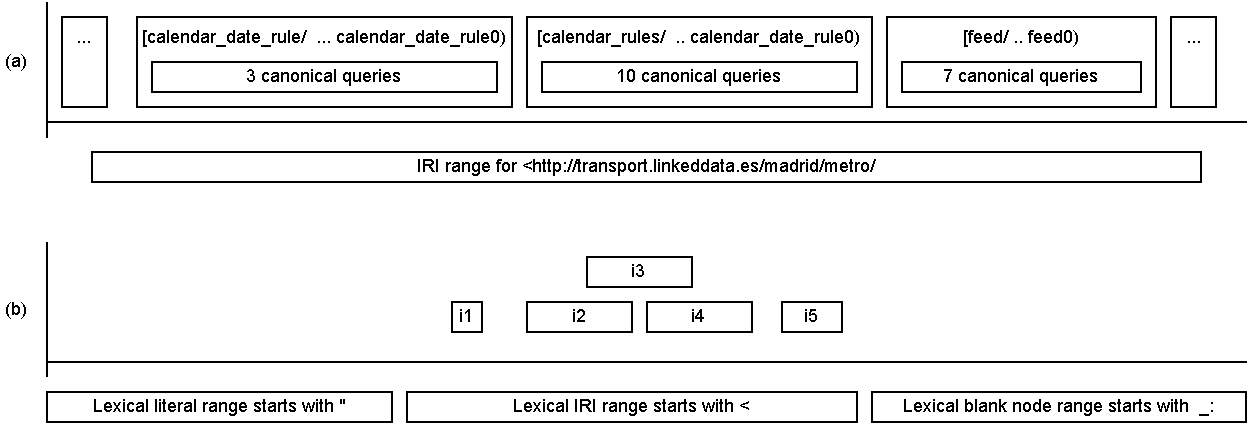
\includegraphics[width=0.95\textwidth]{images/range-partitioning.pdf}
%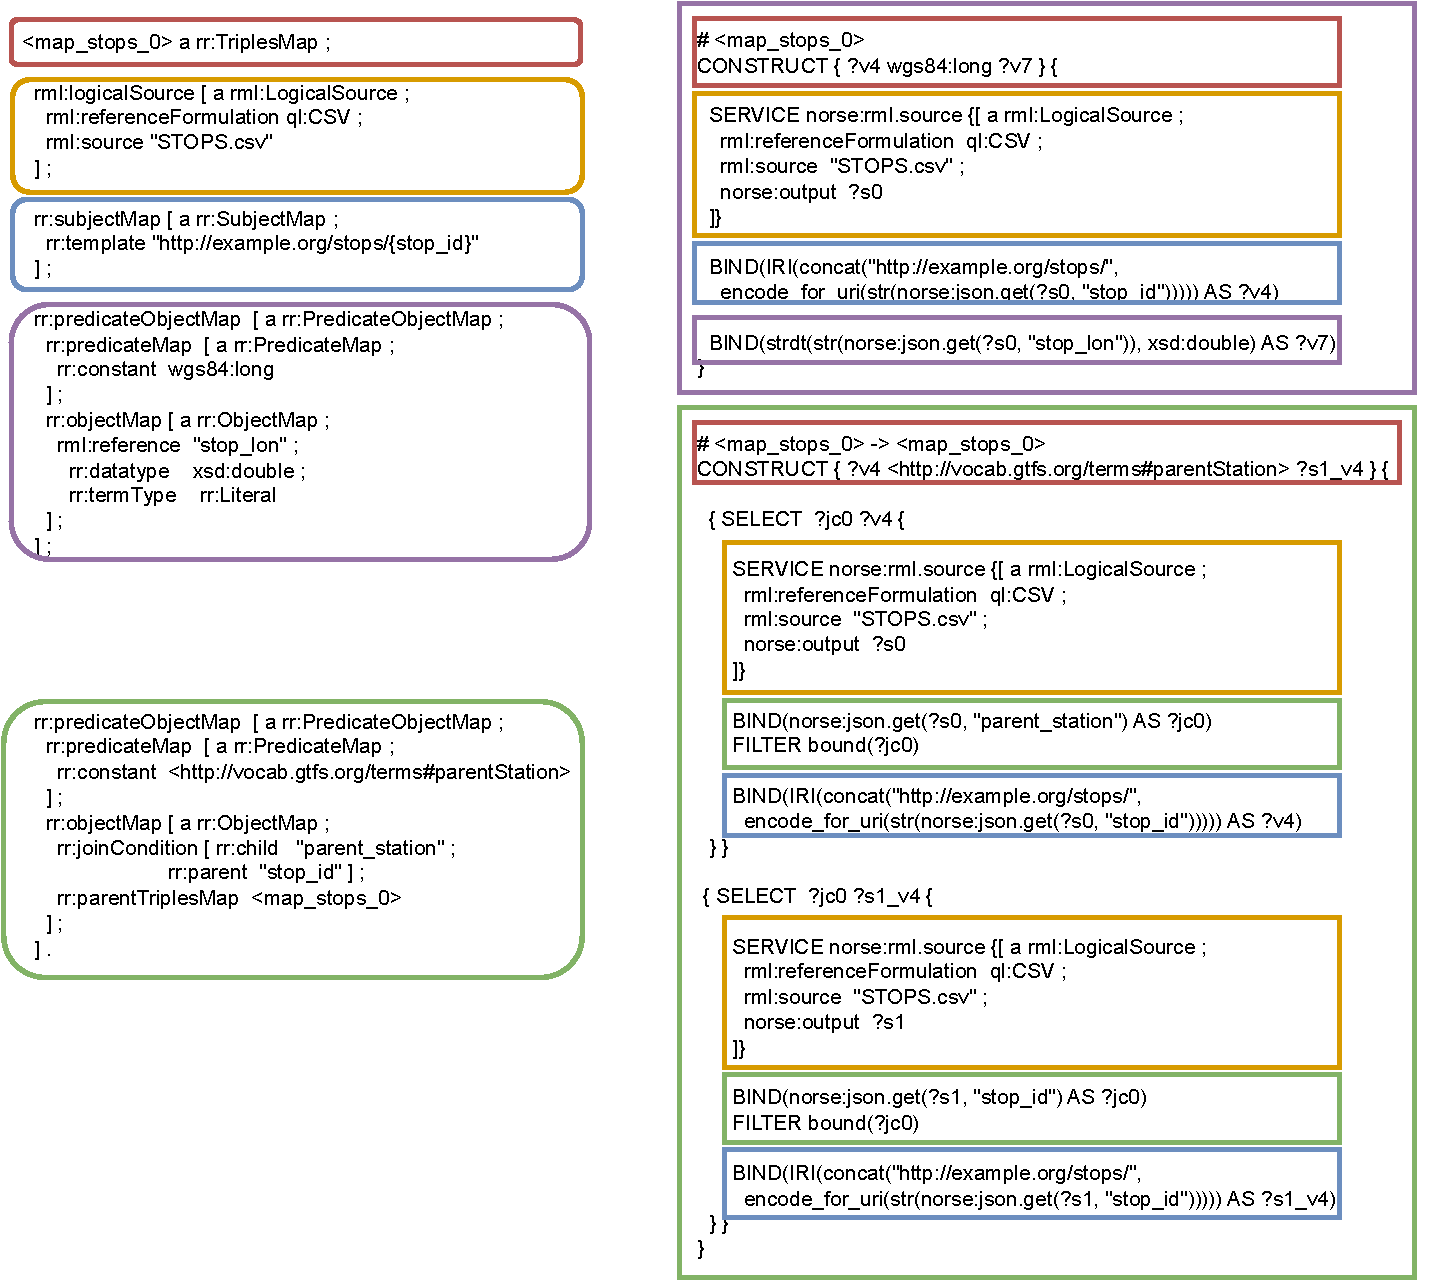
\includepdf[pages=-]{images/rml-to-sparql.pdf}

\caption{(a) An excerpt of the concrete range partitioning of canonical queries obtained from the GTFS-Madrid-Bench mapping based on their produced subjects. (b) An abstract model for RDF Term serialization in N-Quads with example intervals of which some (i3, i4, i5) overlap.}
\label{fig:range-partitioning}
%\caption{Execution time of partitioned queries using SANSA Query 0.9.0 vs Morph KGC 2.4.0}
\end{figure*}


\begin{figure*}[!h]
 \begin{minipage}[t]{0.29\textwidth}
  \centering
  \begin{lstlisting}[language=SPARQL, mathescape=true]
# Query $a$
CONSTRUCT {
  $s_{a_1}$ $p_{a_1}$ $o_{a_1}$
  ...
  $s_{a_n}$ $p_{a_n}$ $o_{a_n}$
} WHERE { $\mathrm{PATTERN_a}$ }

# Query $b$
CONSTRUCT {
  $s_{b_1}$ $p_{b_1}$ $o_{b_1}$
  ...
  $s_{b_m}$ $p_{b_m}$ $o_{b_m}$
} WHERE { $\mathrm{PATTERN_b}$ }
  \end{lstlisting}
%  \caption{listing}{Sub caption}
 \end{minipage}
 \begin{minipage}[t]{0.69\textwidth}
  \centering
  \begin{lstlisting}[language=SPARQL, mathescape=true]
CONSTRUCT { ?s ?p ?o }
WHERE {
  SELECT DISTINCT ?s ?p ?o {
      { $\mathrm{PATTERN}_a$
        LATERAL { { BIND($s_{a_i}, p_{a_i}, o_{a_i}$ AS
          ?s, ?p, ?o) } UNION ... } } # for i in 1..n
    UNION
      { $\mathrm{PATTERN}_b$
        LATERAL { { BIND($s_{b_j}, p_{b_j}, o_{b_j}$ AS
          ?s, ?p, ?o) } UNION ... } } # for j in 1..m
  } ORDER BY ?s ?p ?o
}
  \end{lstlisting}
  %| i \in \{ 1, \ldots, n \}$ 
%  \caption{listing}{Another sub caption}
 \end{minipage}
 \vspace*{-5mm}
 \caption{Generic merge of two (triple-based) CONSTRUCT queries into a single one based on their LATERAL form. The use of DISTINCT and ORDER BY is exemplary to demonstrate the production of truly unique and ordered "inter-query" tuples.}
\label{fig:combine-lateral}
\end{figure*}

%Intutively, it extends SPARQL with support for mapping a single binding to a set of bindings by parameterizing a graph pattern with it. ''flat-Map`` operations 

\subsection{Partitioning Mappings}
In~\Cref{sec:rml-to-sparql} we showed how to translate RML TriplesMaps into a set of SPARQL CONSTRUCT queries. Furthermore, we described how a set of CONSTRUCT queries can be combined into a single one using the novel \texttt{LATERAL} keyword.
This tooling is already sufficient to produce a single CONSTRUCT query from any RML document where DISTINCT and ORDER BY is applied at the top of its SPARQL algebra expression.
However, if it is known that two queries produce disjoint sets of RDF tuples then DISTINCT (and possibly ORDER BY) can be applied independently and their results can be UNION'd. As this leads to operations on fewer data it can significantly improve performance.

In order to achieve this goal it is necessary to obtain a description of the possible set of RDF tuples that can be created from a CONSTRUCT query.
For this purpose we introduce a  model where the set(s) of possible RDF terms (produced by a tuple's component) are represented as intervals.
%Akin to a number line, our interv
%n interval-based
%on a generalized number line.
%It is noteworthy, that the mobindings of a SPARQL result and how to order lines of an N-Quads serialization.
For brevity, we only focus on sorting RDF terms based on the lexical space of their N-Quads serialization.

For example, from an expression such as \lstinline{BIND(IRI(CONCAT("gtfsbench/", ?id)) AS ?x)} we can derive that \texttt{?x} may be any of (1) \texttt{unbound}\footnote{This is the case if \texttt{?id} is not a string because CONCAT only allows for string arguments.} or (2) an IRI with a string value in the interval $[\mathrm{"gtfsbench/"}\; .. \; \mathrm{"gtfsbench0")}$ (under lexicographic order), where $[$ denotes a closed boundary and $)$ an open one, and ``0'' is the successor character of ``/'' in (the ASCII-subset of) UTF-8.

Given a tuple of a construct template, we can thus determine a set of possible values for each of its components.
If the construct template has multiple quads then we can take the component-wise union of the intervals in order to obtain a single description of its producible quads.
% Mention SPAN - so 1 query - 1 interval!
If a variable's set of values is unknown we can gracefully represent it as an interval covering the complete range such as $({-\infty}\; .. \; {+\infty})$.
This way, we can ''project`` every CONSTRUCT query to an interval. \Cref{fig:range-partitioning}~(a) shows a concrete projection based on a subset of the mappings of the GTFS-Madrid-Bench. Each interval corresponds to one or more CONSTRUCT queries.
\Cref{fig:range-partitioning}~(b) shows an abstract example where intervals overlap.
A set of queries with overlapping ranges forms a \emph{partition} and can be merged as shown in~\Cref{fig:combine-lateral} for the sake of applying DISTINCT and ORDER BY.
%\todo{We need to say that we can cluster the CONSTRUCT queries by their interval and then merge them with DISTINCT and ORDER BY applied as described earlier}
Extending this approach to SPARQL is possible but more complex because then the definition of intervals need to consider of the RDF term types and RDF literal datatypes.
%segmentation of the ``number line'' into sub-intervals for each RDF term type and RDF literal datatype.

\subsection{Optimizing DISTINCT by Pulling Up BINDs}
A short-coming of the generated queries is that the DISTINCT operation runs over variables that may be assigned to constants.
By ``pulling'' such definitions up in the algebra DISTINCT can operate on significantly fewer data, which in general increases performance by means of lowering the computational overhead. \Cref{fig:pull-extend} shows an example of rewrite rules we use for optimization. Note, that \texttt{EXTEND} is the algebraic correspondence to the \texttt{BIND} syntax\footnote{\url{https://www.w3.org/TR/sparql11-query/\#sparqlAlgebra}}.
Note, that more sophisticated rules can be devised to split expressions such as \lstinline{CONCAT(const, ...)} into a constant and variable part where the constant part can be pulled up.

%The following algebraic transformation rules allow for "pulling" constant assignments over \texttt{DISTINCT} operations:
%Common variable expression list (commonVel) must be a mapping of variables to constants.
\begin{figure*}[!h]
\begin{itemize}
    \setlength\itemsep{-0.5em}
%    \item Pulling constant assignments up over distinct \texttt{DISTINCT}:
    \item \lstinline{DISTINCT(EXTEND(var, constant, subOp))} $\rightarrow$ \lstinline{EXTEND(var, constant, DISTINCT(subOp))}
    \item \lstinline{UNION(EXTEND(var, constant, left), EXTEND(var, constant, right))} $\rightarrow$
    
    \hspace{1cm}\lstinline{EXTEND(var, constant, UNION(left, right))}
    \item \lstinline{EXTEND(var, non-constant-expr, EXTEND(var, constant, subOp))} $\rightarrow$
    
    \hspace{1cm}\lstinline{EXTEND(var, constant, EXTEND(var, non-constant-expr, subOp))}
\end{itemize}
\vspace*{-5mm}
\caption{A brief excerpt of algebra rewrite rules used to pull EXTEND up.}
\label{fig:pull-extend}
\end{figure*}

\section{Implementation}
\label{sec:implementation}
In this section we provide a brief overview of our related implementations: The NORSE Sparql Extensions, the implementation of the SANSA binding engine (SaBiNe) for evaluating SPARQL on Apache Spark, and finally the RDF Processing Toolking \emph{RPT} which bundles all components together -- including the RML to SPARQL tooling -- into a single command line toolkit.

\paragraph{NORSE SPARQL Extensions and RPT}
JenaX is our project of unofficial extensions for the Apache Jena project. Among its features are the \emph{NORSE} SPARQL extensions. Adding the plugin module as a Maven dependency enhances a Jena-based project with the datatypes and functions for processing CSV, XML and JSON\footnote{\url{https://mvnrepository.com/artifact/org.aksw.jenax/jenax-arq-plugins-bundle}}.

%Committede to upstreaming stable features to Jena or conversely, upstreaming enhancements in order 
\paragraph{Evaluating SPARQL with SANSA and Apache Spark}
Our approach to evaluating SPARQL in Spark is a direct one: A SPARQL result set is represented as an \lstinline{RDD<Binding>}.
%Furthermore, let $\mathrm{Op}$ be the set of SPARQL algebra expressions.
On this basis we present a translation function $[[.]]$ that recursively translates SPARQL algebra operations to operations on (Java) RDDs.
The SANSA Framework thereby provides several features that enable use of functionality from Apache Jena with Apache Spark, such as serializers for SPARQL bindings and algebra expressions. \Cref{lst:sparql-to-spark} shows an excerpt for the evaluation of the SPARQL operations most relevant to RML execution on Apache Spark .

\begin{figure*}[htb]
\begin{itemize}
\setlength\itemsep{-0.5em}
\item \begin{lstlisting}[mathescape=true]
$[[$SERVICE norse:rml.source {[ ... norse:output ?s ]}$]]$ := Create a RDD<Binding> where ?s is bound to records of the specified RML source.
\end{lstlisting}

\item \begin{lstlisting}[mathescape=true]
$[[$FILTER(subOp, expr)$]]$ := $[[$subOp$]]$.filter($\mu \rightarrow \mathrm{exprEval}(\mathrm{expr}, \mu) == true$)
\end{lstlisting}

\item \begin{lstlisting}[mathescape=true]
$[[$JOIN(left, right)$]]$ := $[[$left$]]$.mapToPair($\mu_1 \rightarrow \langle \Pi_J(\mu_1), \mu_1 \rangle$).join($[[$right$]]$.mapToPair($\mu_2 \rightarrow \langle \Pi_J(\mu_2), \mu_2 \rangle$)).map($\langle \mathrm{key}, \langle \mu_1, \mu_2 \rangle \rangle \rightarrow \mu_1 \cup \mu_2$)
\end{lstlisting}
where $J$ is the set of join variables $\mathrm{vars}(\mathrm{left}) \cap \mathrm{vars}(\mathrm{right})$ and $\Pi_J(\mu)$ is the projection of a binding to these variables.
%.filter($(\mu_1, \mu_2) \rightarrow \mathrm{isCompatible}(\mu_1, \mu_2)$)
%and $\mathrm{joinKey}$ is a function that maps each binding to a 
%$\mathrm{vars}(\mathrm{left}) \cap \mathrm{vars}(\mathrm{right})$

\item \begin{lstlisting}[mathescape=true]
$[[$PROJECT(subOp, vars)$]]$ := $[[$subOp$]]$.map($\mu \rightarrow \Pi_{vars}(\mu)$)
\end{lstlisting}

\item \begin{lstlisting}[mathescape=true]
$[[$DISTINCT(subOp)$]]$ := $[[$subOp$]]$.distinct()
\end{lstlisting}

\item \begin{lstlisting}[mathescape=true]
$[[$LATERAL(left, right)$]]$ := if right has no basic graph patterns then
    $[[$left$]]$.mapPartitions($\mu \rightarrow \{ \mu \cup \nu | \forall \nu \in \mathrm{convEval}(\mathrm{subst}(\mathrm{right}, \mu)) \}$)
\end{lstlisting}
where $\mathrm{convEval}$ is conventional SPARQL evaluation into a (Java) collection of bindings rather than a Spark RDD.

\item \begin{lstlisting}[mathescape=true]
$[[$EXTEND(var, expr, subOp)$]]$ := $[[$subOp$]]$.map($\mu \rightarrow \mu \cup \{ \mathrm{var} \rightarrow \mathrm{exprEval}(expr, \mu) \}$)
\end{lstlisting}
\end{itemize}
\vspace*{-5mm}
\caption{Evaluation of selected SPARQL operations with Apache Spark}
\label{lst:sparql-to-spark} 
\end{figure*}

% Issue: The RML sources  actually require this additional project https://github.com/Scaseco/r2rml-api-jena
\paragraph{RDF Processing Toolkit} RPT is the integration project that provides a powerful frontend for both Jena's ARQ and SANSA's SPARQL engines. Both engines support the NORSE and the RML extensions, however only the latter supports parallelization. Example usage of the tooling is shown in~\Cref{lst:usage}.
%and easy-to-use

%# RML to SPARQL Translation
%# Execution
% basicstyle=\scriptsize
\begin{lstlisting}[label=lst:usage, basicstyle=\footnotesize, caption=Example for using RPT to translate and execute RML]
rpt rmltk rml to sparql mapping.rml.ttl > raw.rq
rpt rmltk optimize workload raw.rq --no-order > mapping.rq
JAVA_OPTS="-Xmx16g" rpt integrate mapping.rq --out-file rpt-arq.nt
JAVA_OPTS="-Xmx16g" rpt sansa query mapping.rq --out-file rpt-sansa.nt
\end{lstlisting}


\section{Evaluation}
\label{sec:eval}
We evaluate our approach on the GTFS-Madrid-Bench and one of the largest datasets of SDM-Genomics-Datasets\footnote{The used files are 75percent\_of\_records\_with\_duplicate\_and\_each\_duplicate\_being\_repeated\_20times.csv and 4POM\_Normal.ttl}.
For this purpose we converted the benchmark's RML files to extended SPARQL and ran them using Jena's ARQ and SANSA's SPARQL engine as shown in~\Cref{lst:usage}.
In a first step we evaluated several RML tools on a server with 128GB RAM, AMD Ryzen 9 5950X 16-Core CPU and SSD storage running Ubuntu 20.04.
In order to establish comparability, we used all tools' native unique output feature\footnote{The only exception was Carml for which we appended a \texttt{sort -u} step}. The results for the scale factors 1, 10, 100, 300 are shown in~\Cref{fig:tool-comparison}.
We also attempted to evaluate RocketRML, however we ran into memory issues with it\footnote{\url{https://github.com/semantifyit/RocketRML/issues/44}}.
As for \emph{RMLStreamer}\cite{Haesendonck2019}, on the one hand it requires a Flink setup and on the other hand the initially obtained execution suggested that it lacks the self-join elimination - similar to RMLMapper.

\begin{figure*}[htb]
\centering
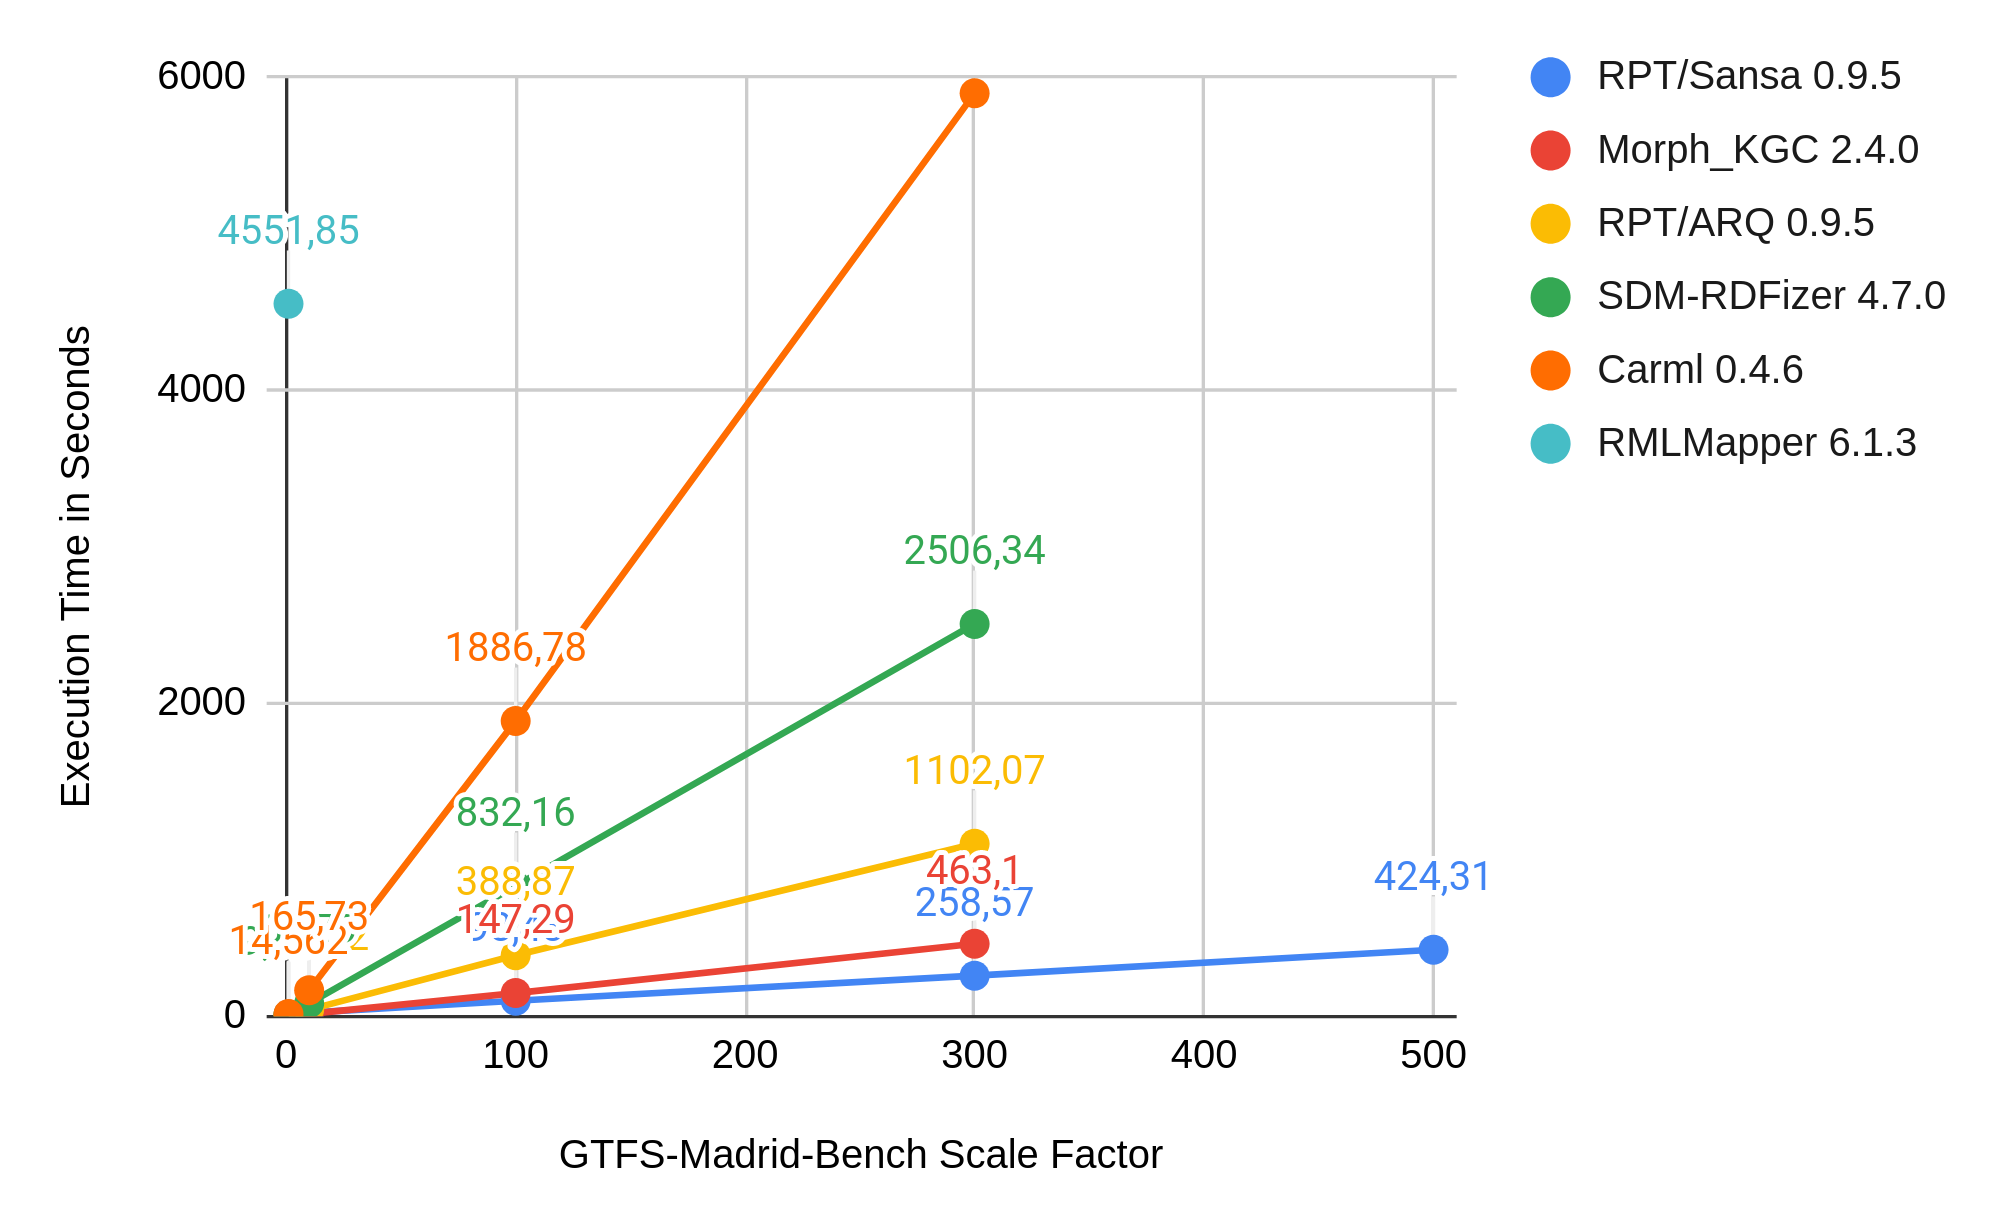
\includegraphics[width=0.7\textwidth]{images/rml-all-tools.png}
%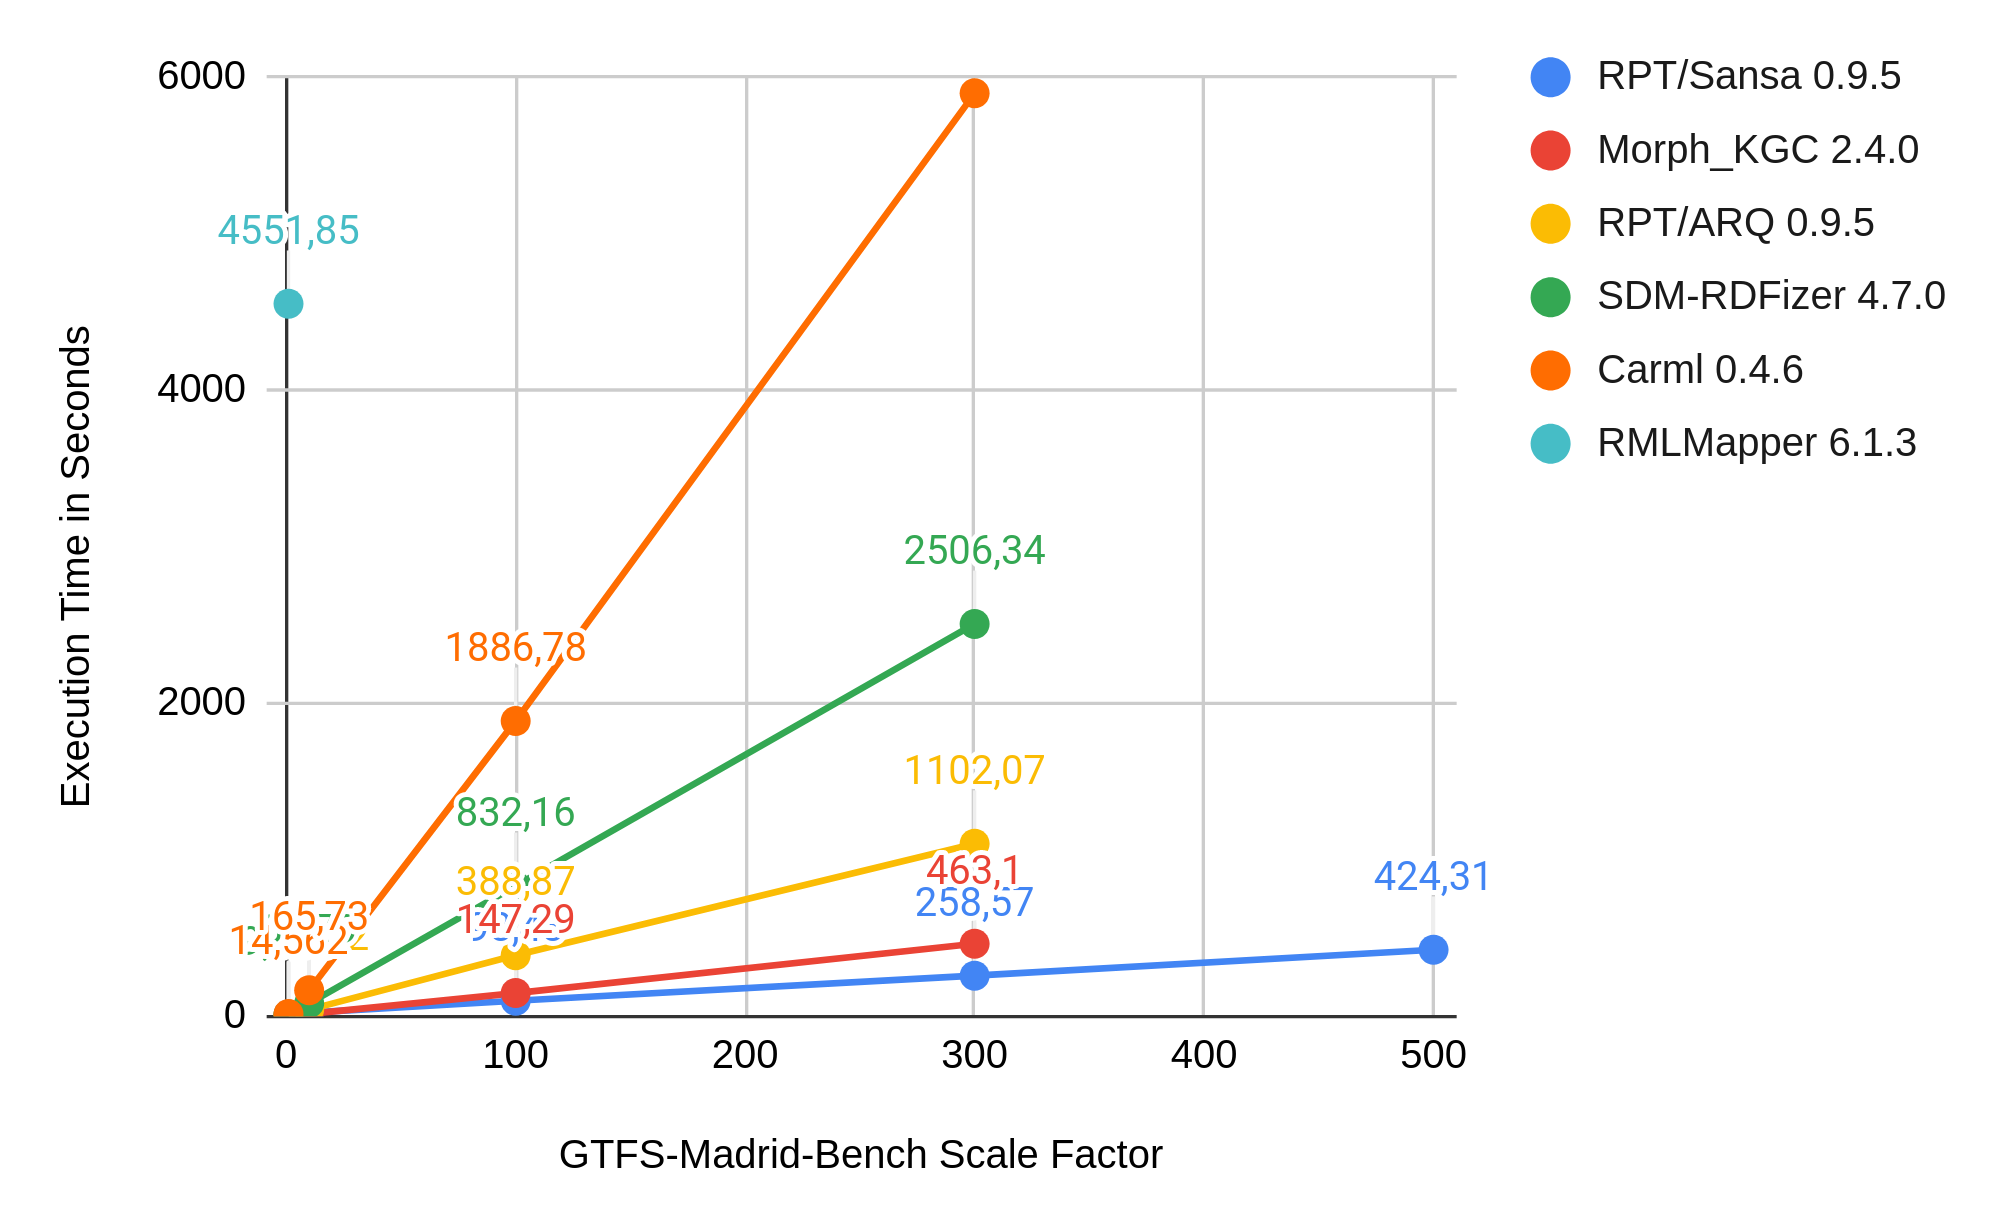
\includepdf[pages=-]{images/rml-all-tools.pdf}
\caption{Comparison of RML mapping tool performance with 128G RAM. On scale factor 500, RPT/ARQ and Morph\_KGC ran out of memory. Carml and SDM-RDFizer were already a magnitude slower on scale factor 300 and were not further evaluated. RMLmapper already exhibited a very high execution time on scale factor 1.}
\label{fig:tool-comparison}
\end{figure*}

In a subsequent step, we evaluated the fastest approaches which are the ones that rely on parallel processing, namely \emph{Morph\_KGC} and \emph{RPT/SANSA}.
%In order to rule out I/O boundness
For this evaluation we needed a machine with more RAM and its specs were: Ubuntu 22.04, 2x Intel(R) Xeon(R) CPU E5-2683 v4 @ 2.10GHz (totalling to 64 threads) and 512GB DDR4 RAM at 2133 MHz. In order to avoid I/O bounds in parallel processing, we performed the experiments for both tools with the benchmark datasets served from the default RAM drive \texttt{/dev/shm}.
With this machine it was possible to scale up to factor 1000.
In addition, we evaluated the tools on the SDM-Genomic-Dataset as this includes a workload that does not involve joins but many duplicates.
As can be seen from~\Cref{fig:eval-chart-execution-time} the execution times for both tools on both workloads converge to scaling linearly.
On smaller sizes Morph\_KGC outperforms RPT/SANSA. With increasing data scale the Apache Spark-based approach gains an advantage. However, on the workload that is mainly about duplicate removal the performance benefit is quite small considering CPU usage:
Morph's average CPU usage in both scenarios is roughly around 400\% whereas RPT/SANSA's is around 4000\%. This means that the latter requires almost 10 times the CPU resources of the former in order to accomplish the same task.
There are many aspects that can cause this significant difference: As a primary source we suspect Apache Spark's processing model for DISTINCT which relies on hash partitioning and shuffling of data which involves (de-)serialization. This introduces a significant overhead when compared to e.g. simply keeping records in an in-memory hash set. Also, Jena introduces additional overhead by having to parse all RDF literals for expression evaluation. 
The benefit is, that invalid literals are reported whenever they are produced during knowledge graph construction.
A performance issue which we detected and fixed during profiling was that Jena would needlessly materialize literals during SPARQL evaluation\footnote{\url{https://github.com/apache/jena/pull/1802}}. Overall, further investigations are necessary to assess the impact of all relevant aspects on the performance in detail.
%the differences in performance in detail.
%substantiate the explanations of the differences.
%This is needed for the evaluation of SPARQL expressions.
%Furthermore, building on an existing SPARQL engine can be both a blessing and a curse: In contrast to Morph\_KGC's current implementation, Jena introduces additional overhead by validating and parsing RDF literals warns about invalid ones.
%. which introduces representations and warns about invalid ones.
%Thereby invalid literals, which occur in the GTFS-Madrid-Bench, further negatively impact performance due to raising internal exceptions.


\begin{figure}
    \centering
    \subfloat[\centering]{{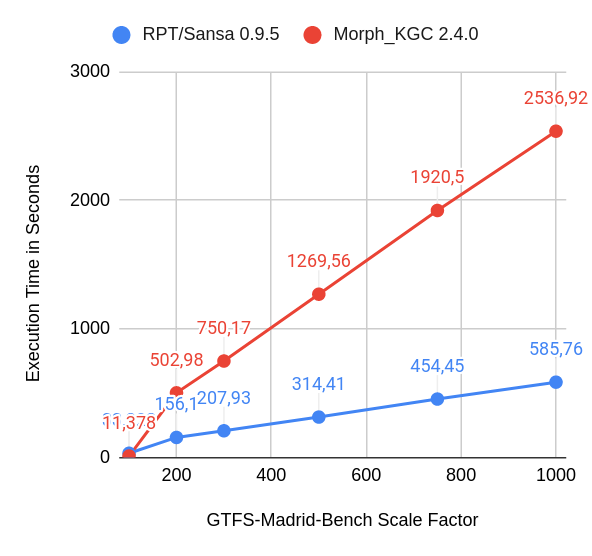
\includegraphics[width=0.47\textwidth]{images/rml-gtfsbench-sansa-vs-morph.png} }}
    \qquad
    \subfloat[\centering]{{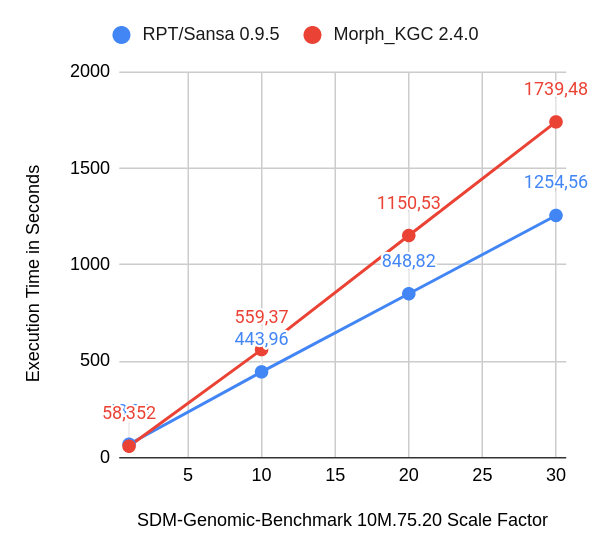
\includegraphics[width=0.47\textwidth]{images/rml-sdm-genomic-morph-vs-sansa.png} }}
    \caption{Execution time of RPT/SANSA and Morph\_KGC with 512G RAM and all data (including temporary) in a RAM disk.}
    \label{fig:eval-chart-execution-time}
\end{figure}


\section{Conclusions and Future Work}
\label{sec:conclusions}
In this work we showed that with the conversion of RML to SPARQL we can leverage suitably enhanced SPARQL engines for the task of knowledge graph construction.
%Just like YARRRML can be converted to RML,  a common ground for query and workload optimization.
We further showed that by transforming CONSTRUCT queries to their ``lateral'' form it is now finally possible to ``merge'' CONSTRUCT queries and remove duplicates which has direct applications in knowledge graph construction.
%Furthermore, using a simple join analysis we can optimize JOINs on Spark by transforming expensive hash joins into cheaper broadcast joins.
Using query workload analysis we can push down DISTINCT operations such that this expensive operation can be computed on smaller RDF graphs.
We showed that the same query workload can be executed on different engines yielding the same result sets however with significantly different performance characteristics. By leveraging a Big Data framework this approach can outperform state of the art approaches.
%In particular, to the best of our knowledge, our Big Data-based approach is the first one to scale to the GTFS1000 benchmark.
We emphasize that as part of this work we contributed the SERVICE extension plugin system as well as minor performance improvements
%as an initial LATERAL implementation
to Apache Jena.
%Our contribution was picked up in Oxigraph and sparked standardization efforts for SPARQL 1.2.
One direction of future work is to optimize the generated SPARQL algebra further as to minimize the amount of data that has to be processed in DISTINCT and ORDER BY operations. Also, as shown in the evaluation, the improved overall performance comes at the cost of significant higher resource usage for which we plan in-depth investigation of the reasons and possible mitigation approaches such as using custom Spark operator implementations.
Furthermore, we identify the need for the standardization of SPARQL for heterogeneous data as this would not only make it possible to transform RML to SPARQL in a truly interoperable way, but also provide a common ground for query and query workload optimization.

%%
%% Define the bibliography file to be used
%\bibliography{ref}


